\documentclass[11pt, dvipsnames, usenames, aspectratio=169]{beamer}
\usepackage{amsmath, amsfonts, amscd, amssymb, amsthm, tikz,pgfplots}

\usepackage{caption}

\usetheme{Madrid}
\usepackage{CoeCollegeSPECIAL}
\usepackage{appendixnumberbeamer}

\bibliographystyle{aer}
\usepackage{natbib}

\setbeamersize{text margin left=10mm,text margin right=10mm} 

\title[Green Development within Urban Areas]{Commercial Green Development within Urban Environments: Theory \& Evidence}
\author{Evan Perry}
\date{August 31, 2021}

\begin{document}

\maketitlepage

%\note{\tiny 
%
%Good evening everyone! My name is Evan Perry, and my summer research supported by the Spellman Fund focused on commercial green development within cities.
%
%}

\begin{frame}{Why Green Buildings? Why Spatially?}

\centering

\begin{tikzpicture}
\fill[rounded corners, crimson] (0,5) rectangle (3, 3) node[pos=.5, white]{\textbf{Scope}};
\fill[rounded corners, lightgray] (3.5,5) rectangle (6.5, 3);
\fill[rounded corners, lightgray] (7,5) rectangle (10, 3);
\draw[rounded corners, thick, white] (0,-1) rectangle (10, 2);
\end{tikzpicture}

\end{frame}

\addtocounter{framenumber}{-1}

\begin{frame}{Why Green Buildings? Why Spatially?}

\centering

\begin{tikzpicture}
\fill[rounded corners, crimson] (0,5) rectangle (3, 3) node[pos=.5, white]{\textbf{Scope}};
\fill[rounded corners, gold] (3.5,5) rectangle (6.5, 3) node[pos=.5, white]{\textbf{Timing}};
\fill[rounded corners, lightgray] (7,5) rectangle (10, 3);
\draw[rounded corners, thick, white] (0,-1) rectangle (10, 2);
\end{tikzpicture}

\end{frame}

\addtocounter{framenumber}{-1}

\begin{frame}{Why Green Buildings? Why Spatially?}

\centering

\begin{tikzpicture}
\fill[rounded corners, crimson] (0,5) rectangle (3, 3) node[pos=.5, white]{\textbf{Scope}};
\fill[rounded corners, gold] (3.5,5) rectangle (6.5, 3) node[pos=.5, white]{\textbf{Timing}};
\fill[rounded corners, teal] (7,5) rectangle (10, 3) node[pos=.5, white]{\textbf{Space}};
\draw[rounded corners, thick, white] (0,-1) rectangle (10, 2);
\end{tikzpicture}

\end{frame}

\addtocounter{framenumber}{-1}

\begin{frame}{Why Green Buildings? Why Spatially?}

\centering

\begin{tikzpicture}
\fill[rounded corners, crimson] (0,5) rectangle (3, 3) node[pos=.5, white]{\textbf{Scope}};
\fill[rounded corners, gold] (3.5,5) rectangle (6.5, 3) node[pos=.5, white]{\textbf{Timing}};
\fill[rounded corners, teal] (7,5) rectangle (10, 3) node[pos=.5, white]{\textbf{Space}};
\draw[rounded corners, thick, white] (0,-1) rectangle (10, 2); 
\draw[thick, ->] (1.5, 3) -- (1.5, 2.1);
\draw[thick, ->] (5, 3) -- (5, 2.1);
\draw[thick, ->] (8.5, 3) -- (8.5, 2.1);
\draw[rounded corners, ultra thick, plum] (0,-1) rectangle (10, 2) node[pos=.5, text width = 9cm]{\textcolor{black}{Commercial green development policy is} \textcolor{crimson}{\textbf{important}} \textcolor{black}{for mitigating climate change and} \textbf{\textcolor{gold}{timely}} \textcolor{black}{-- designing effective policy will require a} \textbf{\textcolor{teal}{spatial perspective}}.
};

\end{tikzpicture}

\end{frame}

\note{

\tiny
I want to start by addressing these questions: why should we care about green buildings, and why should we care about where they're located? 

\bigskip
The first component here to mention is the scope of the problem inherent in our buildings. About 30\% of all greenhouse gas emissions in the US are attributable to buildings. That's a lot. To get to some scenario where we have safe levels of greenhouse gas emissions requires us to address the environmental harm buildings create, and quickly move towards energy-efficient, sustainable buildings. 

\bigskip
A second important component here is timing. If you didn't know, green infrastructure is a pretty hot topic now. There's a solid scientific consensus around the urgency of our climate change response, and building the proper physical infrastructure to do this takes time. Major policy proposals like the Biden administration's American Jobs Plan contain billions of dollars to support the development of a greener infrastructure, especially retrofitting homes and commercial buildings so they're more energy-efficient and environmentally friendly. We need more research to study and support policy, and we need it quickly.

\bigskip
The last piece I want to mention is this spatial component -- why should we care about where these buildings are located? The short answer is to help us design policy and understand the obstacles that these policies face. For instance, if I'm a local policymaker looking to support the development of green buildings, should I try to target investment into certain neighborhoods, or should I create broad incentive programs? Why might some neighborhoods have so few green buildings compared to others? What's inhibiting firms and developers from adopting ``going green" with their buildings? These are important questions that the existing literature isn't suited to address. 

\bigskip
Putting this all together, we can say that ``commercial green development policy is important for mitigating climate change and timely -- designing effective policy will require a spatial perspective."

\vfill
}


\begin{frame}{What Do We Do?}

\begin{enumerate}
	\item \textbf{Theory:} \textit{Create an economic model to describe commercial green development within a city}
	\begin{itemize}
		\item Firms: Chooses a neighborhood, adopt green, and inputs
		\item Developer: Builds green/non-green commercial real estate
	\end{itemize}
	
	\vfill
	\pause
	\item \textbf{Evidence:} \textit{Use data to test the model's predictions}
	\begin{itemize}
		\item Energy Star Program \& Leadership in Energy and Environmental Design (LEED)
		\item SafeGraph Cellphone Data
		\item 33,332 Census tracts (neighborhoods) across 226 Urbanized Areas
	\end{itemize}
\end{enumerate}

\end{frame} 

\note{\tiny

So given this problem, what do we do? When we investigate the literature on commercial green development, we find some basic narratives and stylized facts, but not any real, formalized economic models. Before we can even begin to consider the implications of different policies, we need an economic model. So this is our first goal -- 

\bigskip
We want to create an economic model to describe commercial green development within a city. Right, we're economists, we want something with different agents, variables, parameters, the whole thing.

\bigskip
Now we probably already have some intuition about where green commercial buildings are located and where they aren't. When we go to the data, that intuition is pretty accurate. The point I want to emphasize here is that we aren't interested here in developing some complex theory that yields a shocking result -- we want a model that is formal, precise, and yields some basic insights into a process that otherwise doesn't have much theory behind it. And that's what we do.

\bigskip
While I would be perfectly happy to just make up a bunch of math and call it good, we really should provide some evidence for the theory we develop. So the second piece we want here is to actually take the basic hypotheses out of the model we create and take them to the data. We need to try to verify these empirically.

\vfill
}

\begin{frame}{What Do We Find?}
\begin{columns}
\begin{column}{.48\textwidth}
\begin{enumerate}
	\item \textbf{Theory:} \textit{Forces that drive firms to locate in worker-dense neighborhoods also drive firms to prefer green real estate }
	
	\vspace{1.5cm}
	\item \textbf{Evidence:} \textit{Worker-dense neighborhoods have more green real estate, even when controlling for the total number of workers}
\end{enumerate}
\end{column}
\pause
\begin{column}{.5\textwidth}\centering
\captionof{figure}{Green Commercial Buildings,\\ Des Moines}
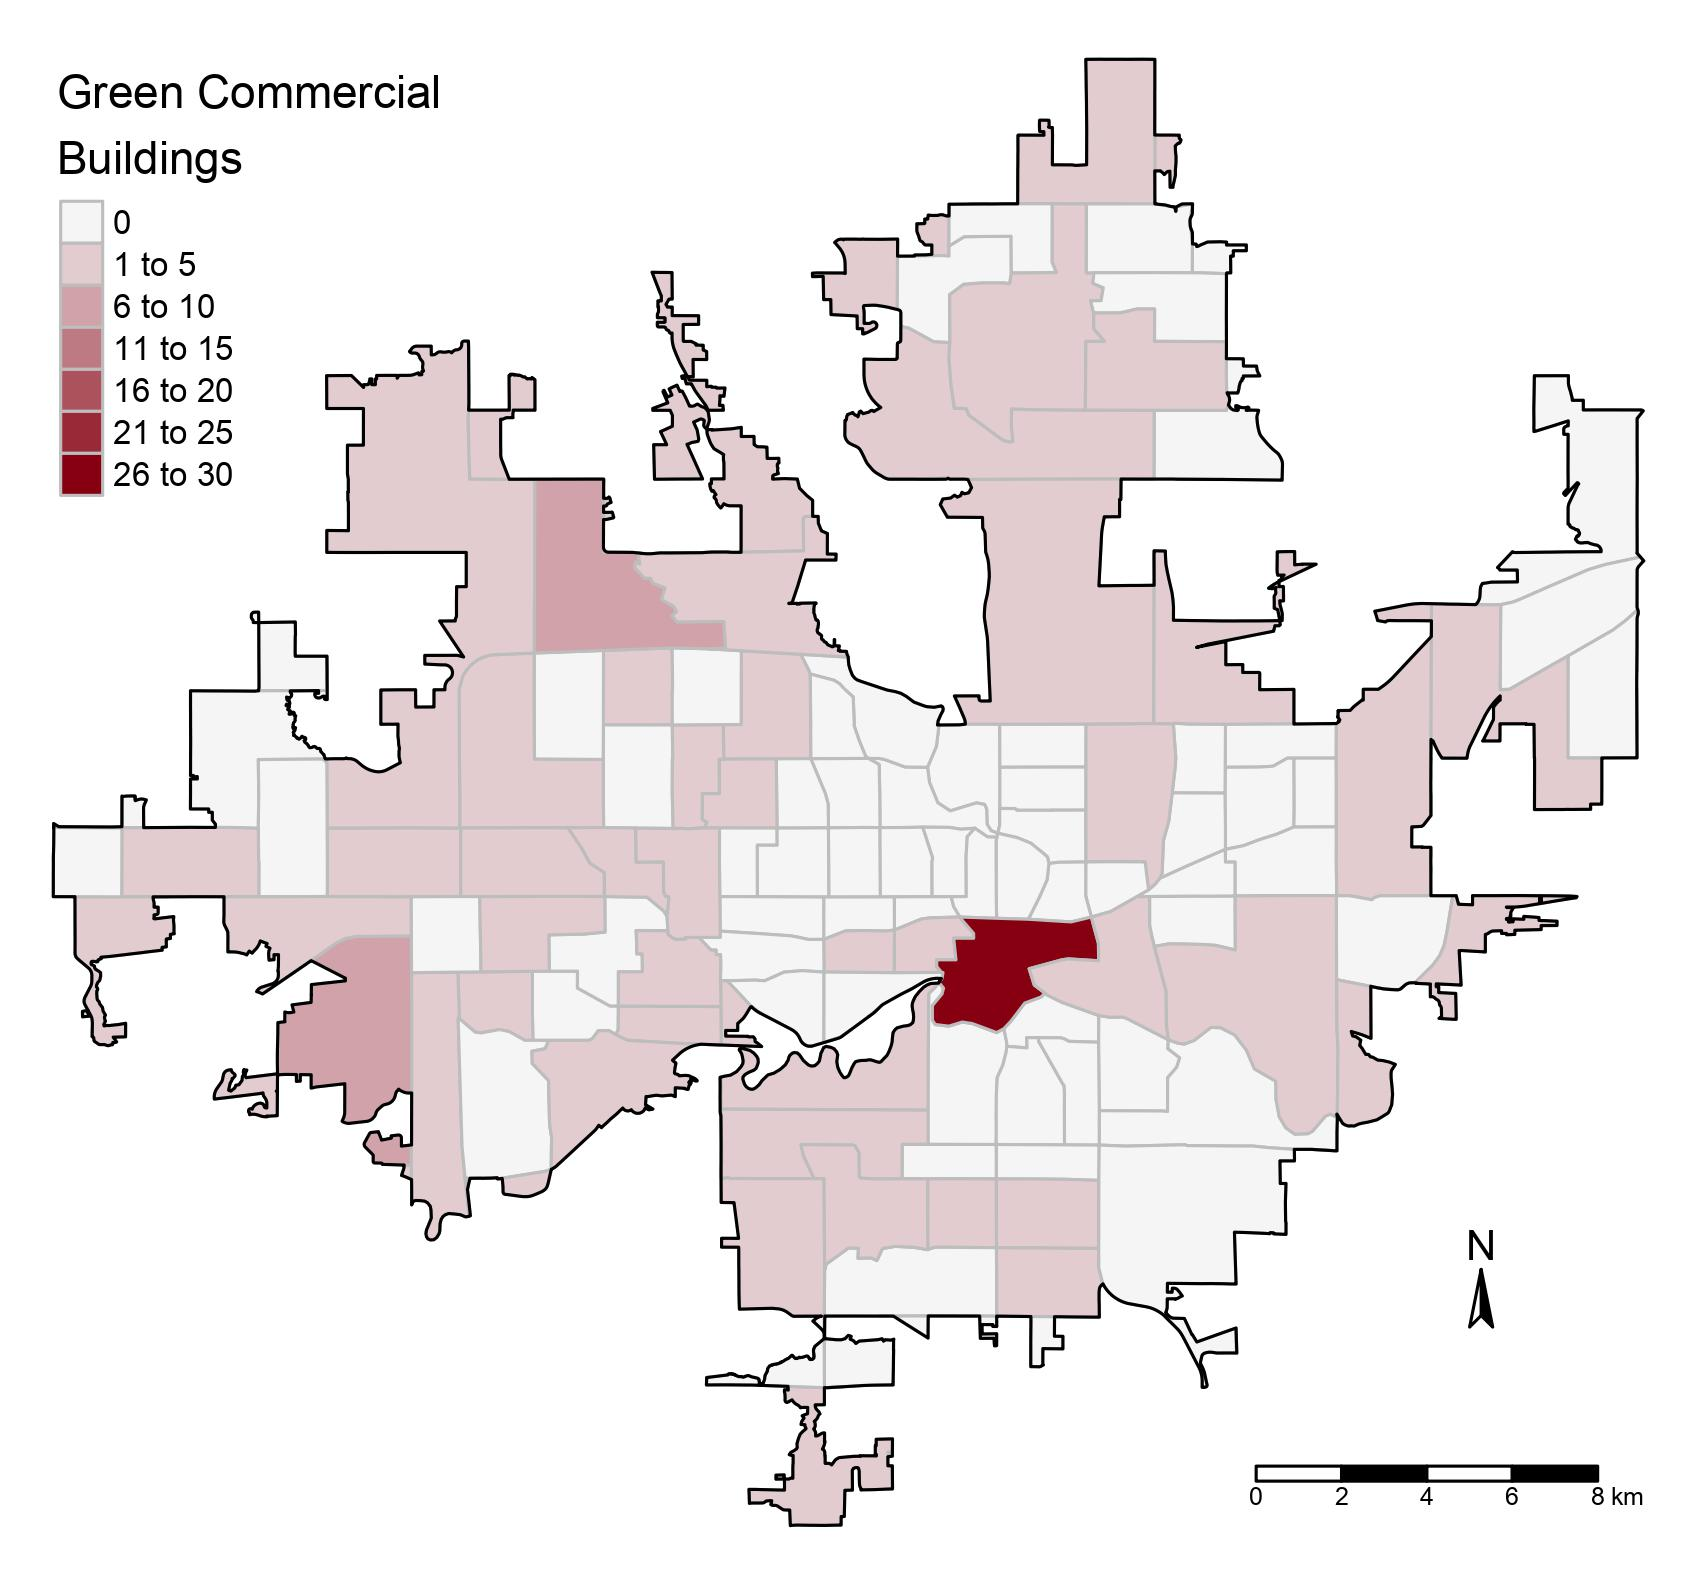
\includegraphics[width = 0.9\textwidth]{0001.jpg}
\end{column}
\end{columns}

\end{frame}

\note{\tiny

Lastly, what do we find?

\bigskip
On the theory side, we make this connection between the pieces behind a firm's decision to locate and a firm's decision to occupy a green building. Specifically, we find that the ``forces that drive firms to locate in worker-dense neighborhoods," think like downtown, ``also drive firms to prefer green real estate.” We find that different types of firms decide to locate in more or less worker-dense neighborhoods, and this selection process means that green buildings are proportionately more common in these ``downtown" areas.

\bigskip
Empirically, we go to the data and try to assess whether or not this has any merit, and we find that it does. ``Worker-dense neighborhoods have more green real estate, even when controlling for the total number of workers."

\bigskip
To illustrate this, here's a map of the number of green buildings by Census tract or neighborhood in Des Moines. We can see pretty clearly that this central downtown neighborhood has far more green commercial buildings than any other neighborhood in the city, and even when we adjust for the number of workers, similar to the number of commercial buildings, we still see this area stand out. Empirically, we're able to generalize this to not just Des Moines, but to hundreds of cities across the US.

\bigskip
All in all, we contribute to this existing literature and research by developing this new model for green commercial development, and we establish that its basic predictions fit with the real world. This model could support future research into various green development policies and programs.

\vfill
}

\begin{frame}
\Large\textcolor{crimson}{\textbf{Thank You}}
\end{frame}

\end{document}